\chapter{Cas d'utilisations}

\section{Diagramme}

\begin{figure}
  \centering
  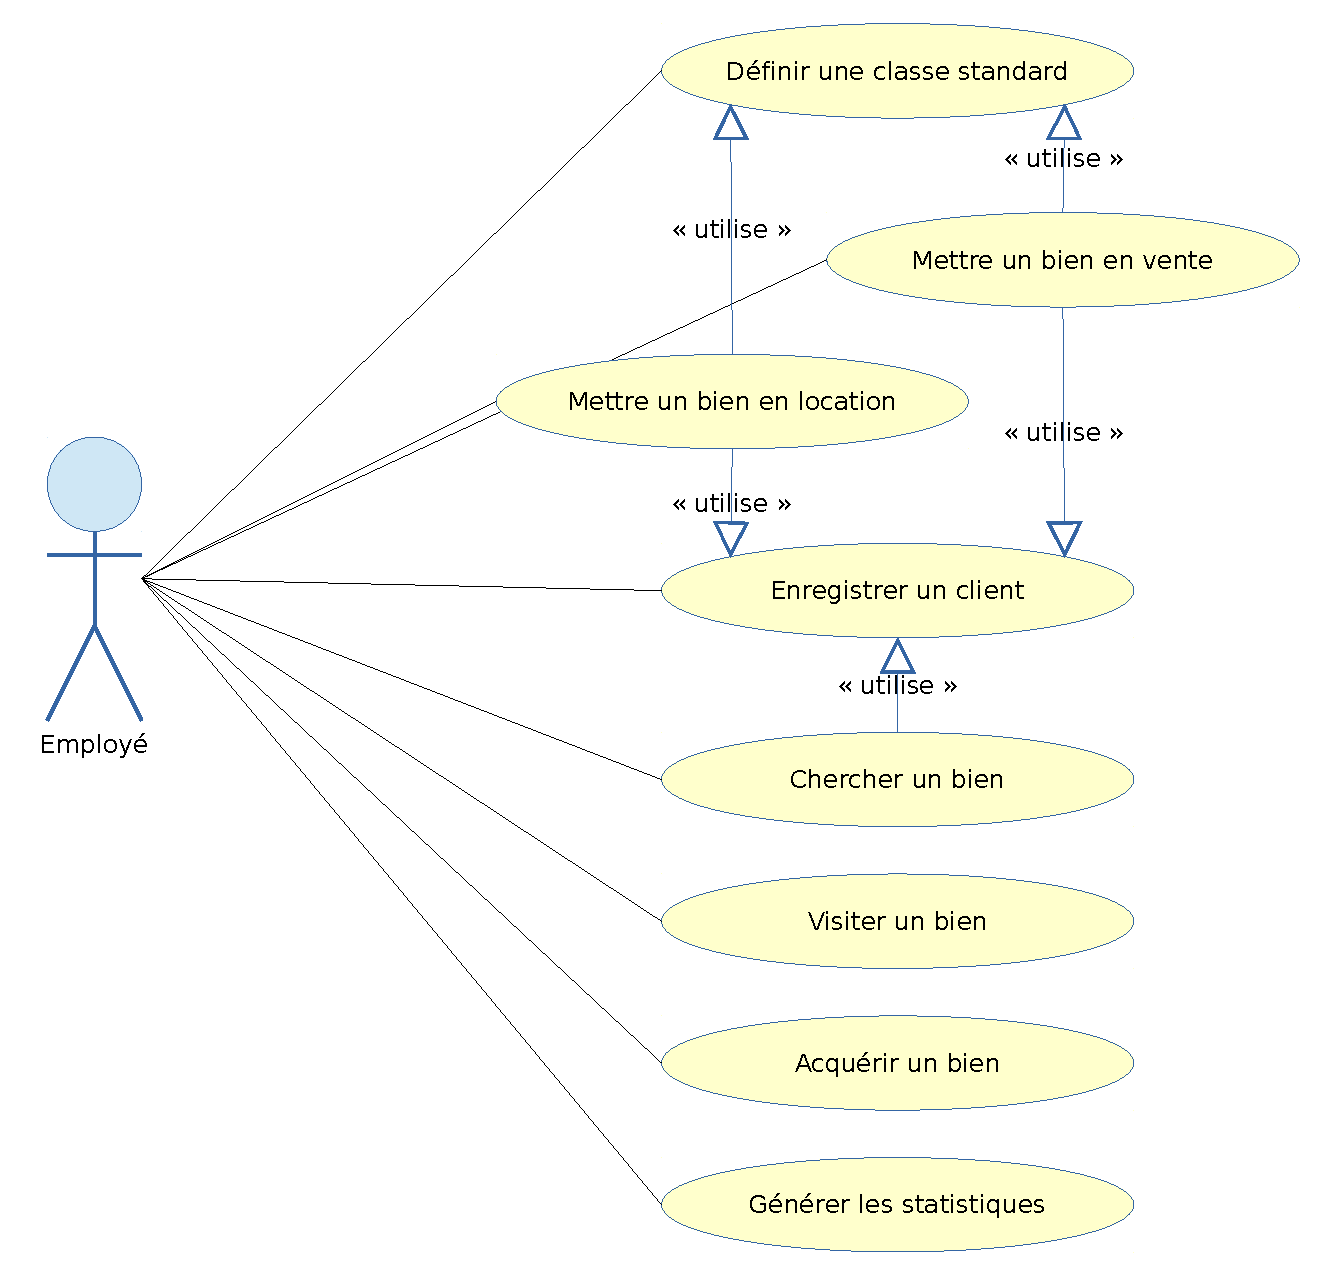
\includegraphics[width=0.95\textwidth]{IMG/uc}
  \caption{Cas d'utilisations}
  \label{img_uc}
\end{figure}

La figure \refpage{img_uc} illustre les cas d'utilisations du projet.

\section{Scénarios}

\subsection{Définir une classe standard}

L'employé va créer une classe et définir les paramètres que les biens devront remplir pour en faire partie.

\subsection{Mettre un bien en vente}

Le bien à mettre en vente doit appartenir à un client enregistré dans le système. S'il s'agit d'un nouveau client, ce dernier sera d'abord enregistré. L'employé va enregistrer les différents paramètres du bien dans le système. Les paramètres à enregistrer dépendront du type de bien. Le bien se verra attribuer une ou plusieurs classes d'après ses paramètres.

\subsection{Mettre un bien en location}

Le bien à mettre en location doit appartenir à un client enregistré dans le système. S'il s'agit d'un nouveau client, ce dernier sera d'abord enregistré. L'employé va enregistrer les différents paramètres du bien dans le système. Les paramètres à enregistrer dépendront du type de bien. Le bien se verra attribuer une ou plusieurs classes d'après ses paramètres.

\subsection{Enregistrer un client}

L'employé va enregistrer les données du client dans le système. Les données à enregistrer sont le nom et le numéro de téléphone.

S'il s'agit d'un offrant, l'employé enregistrera également le téléphone professionnel ainsi que les heures heures auxquelles le client est accessible sur chaque numéro.

Sinon, le client sera associé à une série de classes standards qui correspondent aux types de biens qu'il recherche. Une recherche de bien sera ensuite automatiquement exécutée.

\subsection{Chercher un bien}

Le système va générer la liste de tous les biens correspondants aux classes standard d'un client donné.

\subsection{Visiter un bien}

Pour chaque bien obtenu par la recherche et retenu pas le client, le système va fournir toutes les informations. Si le client est intéressé par une visite, différentes dates et heures seront proposées par le système. L'employé et le client se mettent d'accord sur une date et une heure précise qui sera enregistrée dans le système. Un responsable de l'agence sera également assigné pour effectuer la visite.

\subsection{Acquérir un bien}

Lorsqu'un client est intéressé par un bien, une proposition sera envoyée au propriétaire. Si ce dernier l'accepte, un contrat sera émis entre le propriétaire et l'acquéreur via l'agence.

Il est possible que le propriétaire n'accepte pas l'offre de l'acquéreur. Ce refus peut être définitif, ou déboucher sur une négociation qui aboutira à l'acceptation d'une offre.

\subsection{Générer les statistiques}

De manière à fournir régulièrement des informations pertinentes au service de prospection, le service d'enregistrement des demandes produit un document statistique récapitulant les différents types de demandes. Cet état statistique est généré en fin de semaine ou dès que 100 demandes sont enregistrées. Ces statistiques seront mise à disposition des employés du service de prospection.

\section{Rapport}

J'ai ici défini les cas d'utilisations principaux résultant de l'exercice courant de l'agence immobilière. Nous devrions également envisager différents cas comme la modification des informations du système (mise à jour et suppression des classes standard, des biens, des clients, etc.). Toutefois, cela alourdirait sensiblement le diagramme sans y apporter de réelle plus-values. En effet, elles sont généralement implicites.